\section{Part 3 - Multivariable control}
\subsection{Problem 1}
Here, we are to find the systems matrices $\boldsymbol{A}$ and
$\boldsymbol{B}$. Trivially, they are:

\begin{equation}
  \boldsymbol{A} = \begin{bmatrix}
    0 & 1 & 0 \\
    0 & 0 & 0 \\
    0 & 0 & 0 \\
  \end{bmatrix}, \hspace{0.5cm}
  \boldsymbol{B} = \begin{bmatrix}
    0 & 0 \\
    0 & K_1 \\
    K_2 & 0 \\
  \end{bmatrix}
\end{equation}

\subsection{Problem 2}
First, we are to examine the controllability of the system. We do that
by finding the controllability matrix $\boldsymbol{\mathcal{C}}$ of
the system, and see whether it has full rank or not:

\begin{equation}
  \boldsymbol{\mathcal{C}} = \begin{bmatrix}
    \boldsymbol{B} & \boldsymbol{AB}
  \end{bmatrix}
  =
  \begin{bmatrix}
    0 & 0 & 0 & K_1 \\
    0 & K_1 & 0 & 0 \\
    K_2 & 0 & 0 & 0 \\
  \end{bmatrix}
\end{equation}
which has full rank: $rank(\bm{\mathcal{C}}) = 3$, and is thus
controllable.

Second, we are to implement a LQR controller with reference
feed-forward, $u = \bm{Pr}-\bm{Kx}$. K is derived from the Matlab lqr
function, which requires the A and B matrices, in addition to
weighting matrices Q and R. When finding appropriate Q and R matrices,
Byrson's rule guided the first iteration. The rule states:

\begin{equation}
  Q_{ii} = \frac{1}{\text{maximum acceptable value of }x_i^2}
\end{equation}
\begin{equation}
  R_{jj} = \frac{1}{\text{maximum acceptable value of }u_j^2}
\end{equation}
where $x_i$ represents the $i^{th}$ state and $u_j$ represents the
$j^{th}$ input. All other entries to Q and R are 0. This resulted
in: \begin{equation}
  Q =
  \begin{bmatrix}
    1/(\pi/8)^2 & 0          & 0 \\
    0 &          1/(\pi/2)^2 & 0 \\
    0 &          0          & 1/(\pi/8)^2 \\
  \end{bmatrix}
  \qquad
  R =
  \begin{bmatrix}
    1 & 0 \\
    0 & 1 \\
  \end{bmatrix}
\end{equation}
We chose these initial values to have a small range of motion in
pitch, a large max speed in pitch to better control the pitch and a
relatively slow maximum speed in elevation. Furthermore, both inputs
max value is 1.

After tuning, the following Q and R matrices seemed to perform with
the quickest response without large overshoots:
\begin{equation}
  Q =
  \begin{bmatrix}
    60 & 0   & 0 \\
    0  & 0.01 & 0 \\
    0  & 0   & 100 \\
  \end{bmatrix}
  \qquad
  R =
  \begin{bmatrix}
    1 & 0 \\
    0 & 1 \\
  \end{bmatrix}
\end{equation}
A higher value for $q_{1,1}$ yields a more oscillatory pitch behavior,
while a lower value yields a slower response. As for $q_{2,2}$ a
higher value slowed the pitch response. With $q_{3,3} > 100$ the
system becomes difficult to control.
\todo[inline]{Explain why the system becomes difficult to control}

$\boldsymbol{P}$ is defined such that as time goes to infinity, our
states $\tilde{p}$ and $\dot{\tilde{e}}$ tend to their reference
values $\tilde{p}_c$ and $\dot{\tilde{e}}_c$. This happens when
$\dot{\boldsymbol{x}} = 0$, as the system reaches a stable equilibrium
around the reference values:

\begin{align*}
  \dot{\boldsymbol{x}} &= \boldsymbol{Ax} + \boldsymbol{Bu} \\
                       &= \boldsymbol{Ax} +
                         \boldsymbol{B}(\boldsymbol{Pr} -
                         \boldsymbol{Kx}) \\
                       &= (\boldsymbol{A}-\boldsymbol{BK})\boldsymbol{x}
                         + \boldsymbol{BPr} = 0
\end{align*}
When $\boldsymbol{\dot{x}} = 0$, our $\boldsymbol{x}$ has reached its
final value and we define $\boldsymbol{x} = \boldsymbol{x_\infty}$:

\begin{align*}
  (\boldsymbol{BK} - \boldsymbol{A})\boldsymbol{x_\infty} = \boldsymbol{BPr} \\
  \Leftrightarrow \boldsymbol{x_\infty} = (\boldsymbol{BK} - \boldsymbol{A})^{-1}\boldsymbol{BPr} \\
  \Rightarrow \boldsymbol{y_\infty} = \boldsymbol{Cx_\infty} = \boldsymbol{C}(\boldsymbol{BK} - \boldsymbol{A})^{-1}\boldsymbol{BPr}
\end{align*}
We see that our output $\boldsymbol{y_\infty}$ is equal to our reference $\boldsymbol{r}$ when:
\begin{equation}
  \boldsymbol{P} = [\boldsymbol{C}(\boldsymbol{BK} - \boldsymbol{A})^{-1}\boldsymbol{B}]^{-1}
\end{equation}
Therefore, we now have
\begin{align*}
  \lim_{t\to\infty}\boldsymbol{y}(t) = \boldsymbol{y_\infty} =
  \begin{bmatrix}
    \tilde{p} \\
    \dot{\tilde{e}}
  \end{bmatrix}
  =
  \begin{bmatrix}
    \tilde{p}_c \\
    \dot{\tilde{e}}_c
  \end{bmatrix}
  = \boldsymbol{r},
\end{align*}
which is what we wanted.
\subsection{Problem 3}
With integral effect, the new state space matrices become:
\begin{equation}
  \boldsymbol{A} = \begin{bmatrix}
    0 & 1 & 0 & 0 & 0\\
    0 & 0 & 0 & 0 & 0\\
    0 & 0 & 0 & 0 & 0\\
    1 & 0 & 0 & 0 & 0\\
    0 & 0 & 1 & 0 & 0\\
  \end{bmatrix}, \hspace{0.5cm}
  \boldsymbol{B} = \begin{bmatrix}
    0 & 0 \\
    0 & K_1 \\
    K_2 & 0 \\
    0 & 0 \\
    0 & 0 \\
  \end{bmatrix}, \hspace{0.5cm}
  \boldsymbol{C} = \begin{bmatrix}
    1 & 0 & 0 & 0 & 0\\
    0 & 0 & 1 & 0 & 0\\
  \end{bmatrix}
\end{equation}

The matrices used to calculate the controllers gains, Q and R, also needed to be updated:

\begin{equation}
  Q =
  \begin{bmatrix}
    60 & 0   & 0  & 0 & 0 \\
    0  & 0.01 & 0  & 0 & 0 \\
    0  & 0   & 100 & 0 & 0 \\
    0  & 0   & 0  & 100 & 0 \\
    0  & 0   & 0  & 0 & 30 \\
  \end{bmatrix}
  \qquad
  R =
  \begin{bmatrix}
    1 & 0 \\
    0 & 1 \\
  \end{bmatrix}
\end{equation}

Without integral effect, the system could track pitch without much of
a problem. But the elevation rate had a noticeable deviation in the
ranges of elevation not close to our linearization point
$\dot{\tilde{e}} = 0$.

With integral effect, this deviation in elevation rate is
asymptotically removed. This means that with a zero Y output from our
joystick, we see a corresponding zero elevation rate, and the
elevation angle stays asymptotically constant also for angles not
close to its linearization point.

\begin{figure}[hbp]
\caption{LQR Controller with no Integral Effect}
	\centering
		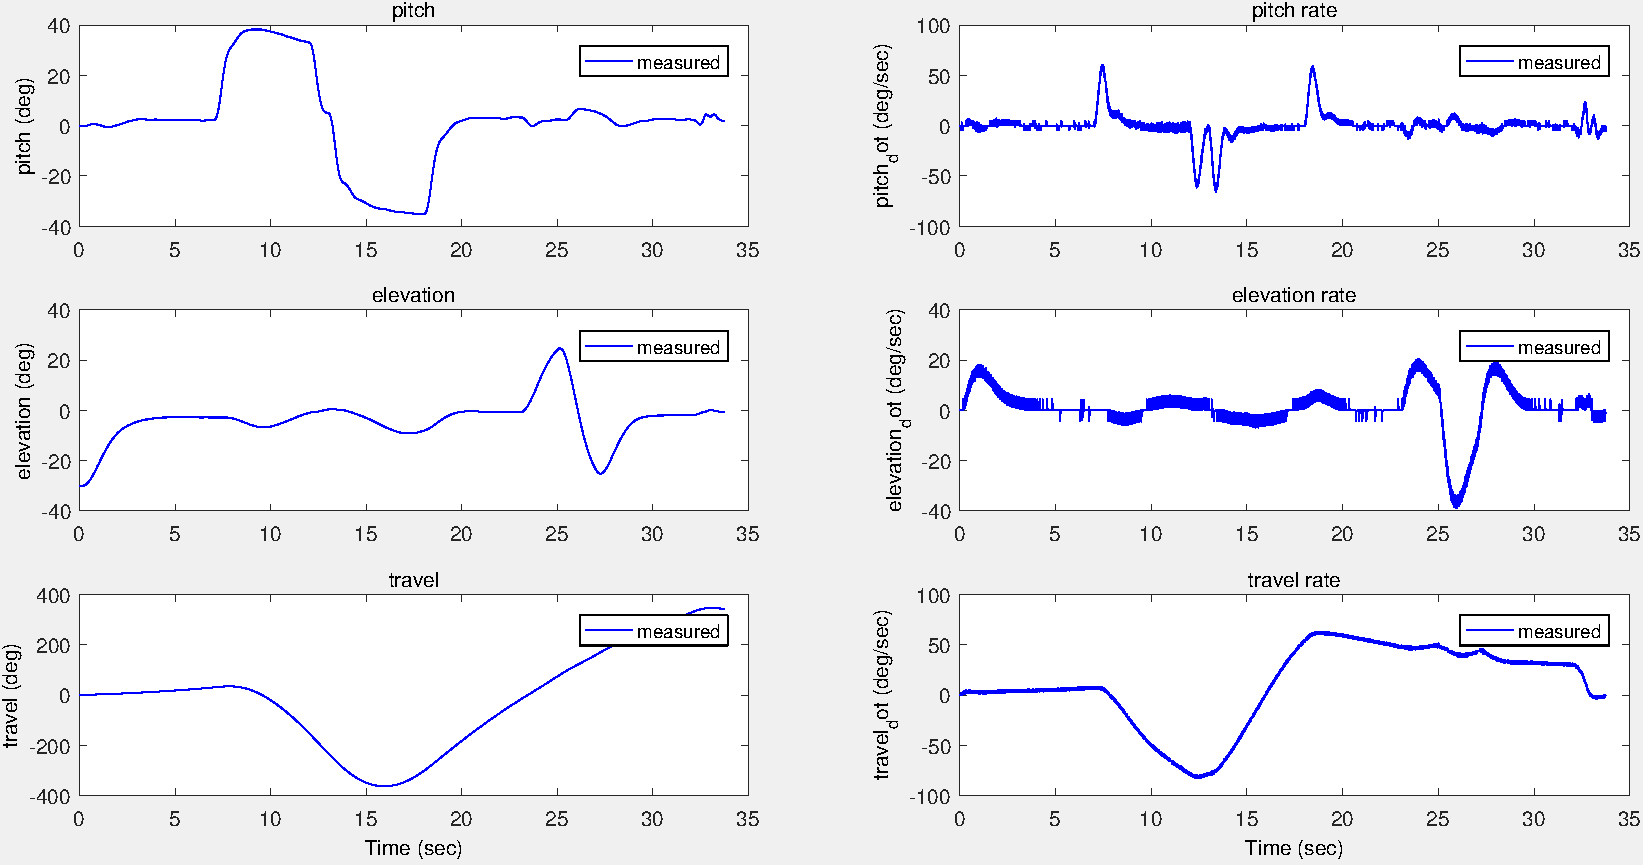
\includegraphics[scale =0.4]{images/532_LQR_NoEstimator.pdf}
	\label{fig:LQR_noEstimator}
\end{figure}

\begin{figure}
\caption{LQR Controller with Integral Effect}
	\centering
		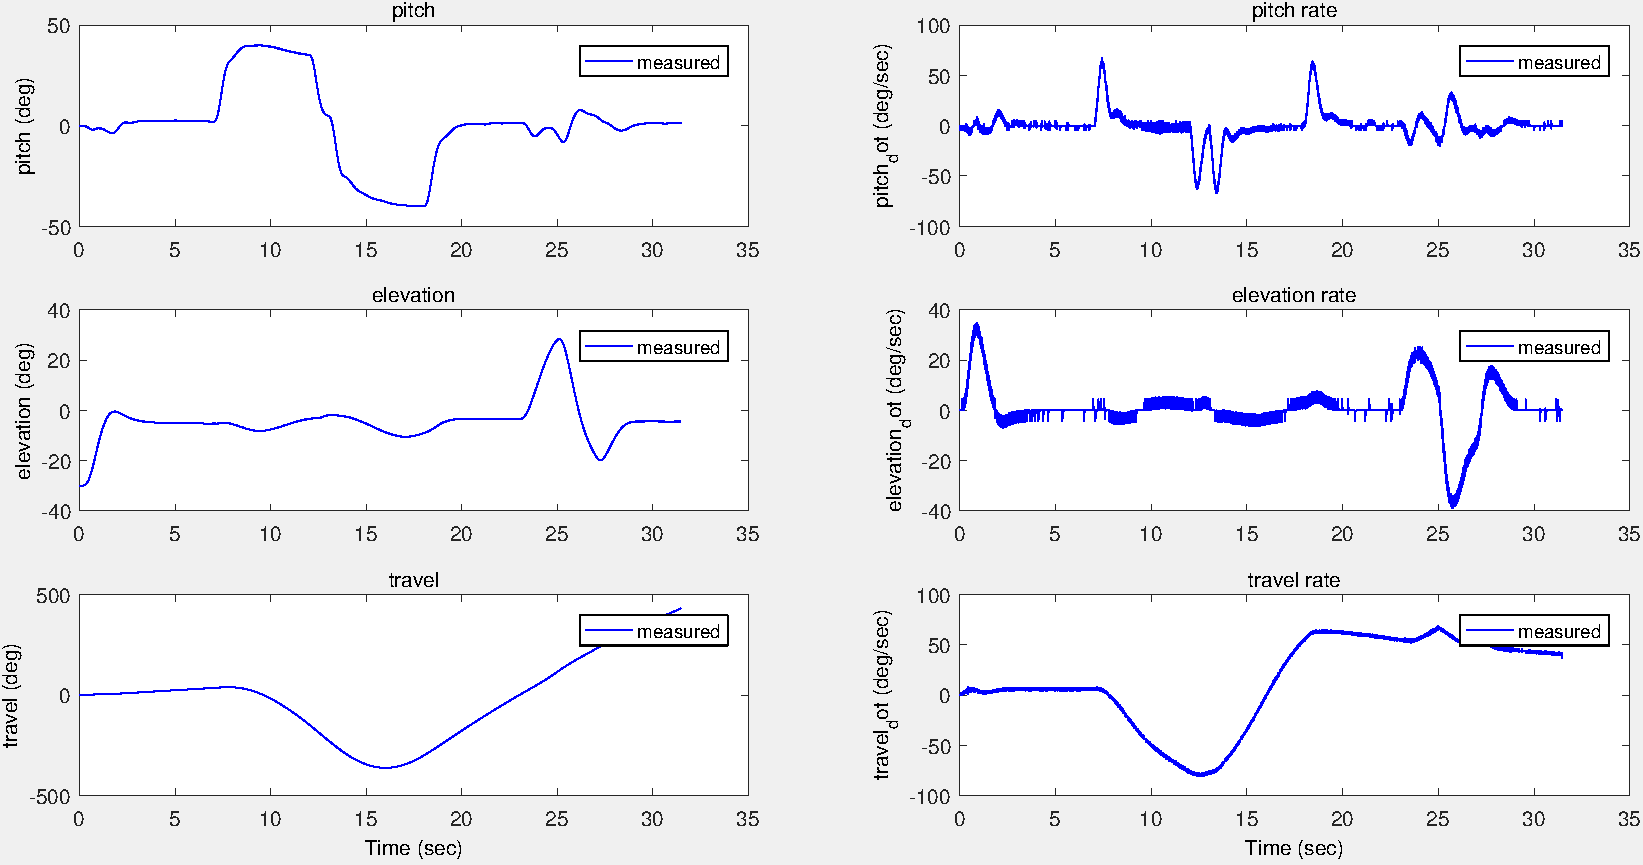
\includegraphics[scale =0.4]{images/533_LQRIntegralEffect_NoEstimator.pdf}
	\label{fig:LQRIntegralEffect_noEstimator}
\end{figure}

\begin{figure}
\caption{Input for no Integral Effect}
	\centering
		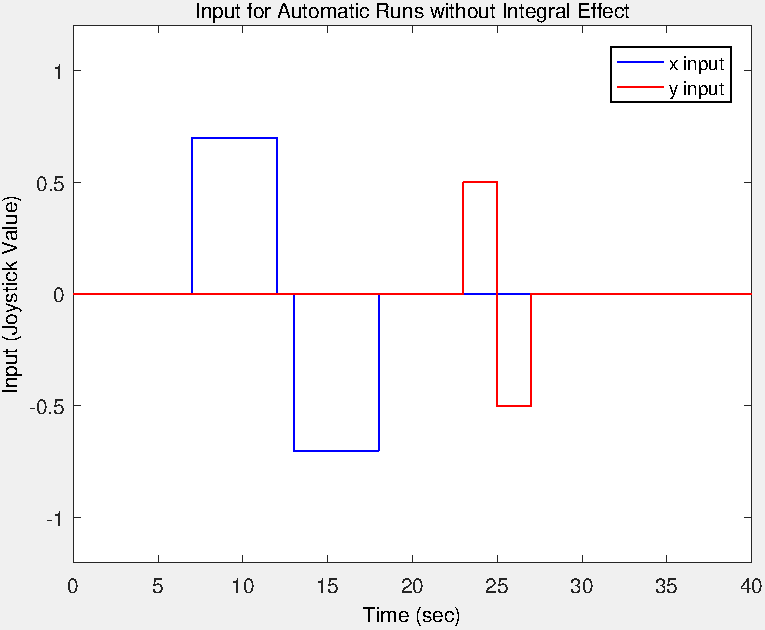
\includegraphics[scale =0.6]{images/input_noIntegralEffect.pdf}
	\label{fig:Input_noIntegralEffect}
\end{figure}

\begin{figure}
\caption{Input with Integral Effect}
	\centering
		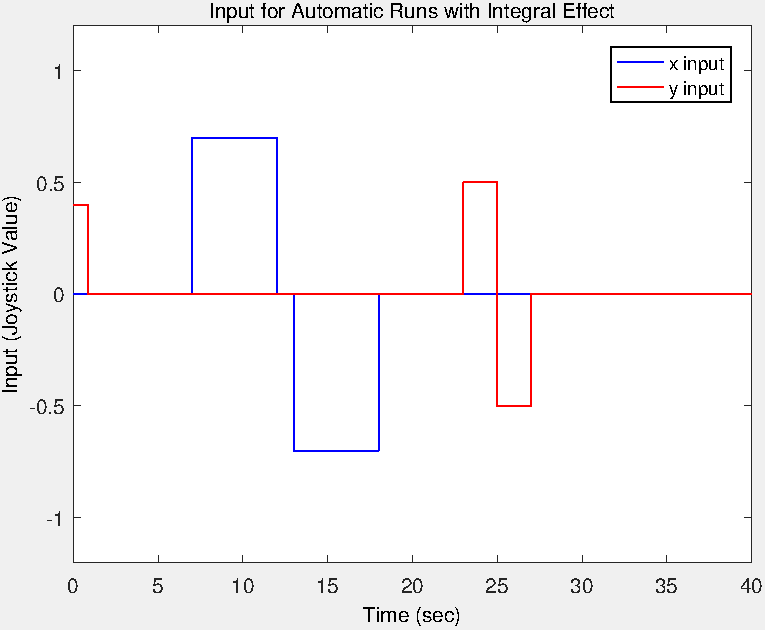
\includegraphics[scale =0.6]{images/input_IntegralEffect.pdf}
	\label{fig:Input_IntegralEffect}
\end{figure}
%%% Local Variables:
%%% mode: latex
%%% TeX-master: "report_main"
%%% End:
